\documentclass[dvipdfmx,11pt,notheorems]{beamer}
%%%% 和文用 %%%%%
\usepackage{bxdpx-beamer}
\usepackage{pxjahyper}
\usepackage[dvipdfmx]{movie15_dvipdfmx}
\usepackage{minijs}%和文用
\usepackage{listings,jlisting} % プログラムの表示用
\usepackage{type1cm}
\renewcommand{\kanjifamilydefault}{\gtdefault}%和文用

%%%% スライドの見た目 %%%%%
\usetheme{Boadilla}
\usecolortheme{seahorse}
\usefonttheme{professionalfonts}
\setbeamertemplate{frametitle}[default][center]
\setbeamertemplate{navigation symbols}{}
\setbeamercovered{transparent}%好みに応じてどうぞ)
\setbeamertemplate{footline}[page number]
\setbeamerfont{footline}{size=\normalsize,series=\bfseries}
\setbeamercolor{footline}{fg=black,bg=black}

\setbeamercolor{white-cyan1}
{fg=white,bg=cyan!80!black}
\setbeamercolor{white-cyan2}
{fg=white,bg=cyan!60!black}

%フラットデザイン化
\setbeamertemplate{blocks}[rounded] % Blockの影を消す
%Beamer色設定
\definecolor{UniBlue}{RGB}{0,150,200}
\definecolor{AlertOrange}{RGB}{255,76,0}
\definecolor{AlmostBlack}{RGB}{38,38,38}
\setbeamercolor{structure}{fg=UniBlue} % 見出しカラー
\setbeamercolor{block title}{fg=UniBlue!50!black} % ブロック部分タイトルカラー
%%%%

%%%% 定義環境 %%%%%
\usepackage{amsmath,amssymb}
\usepackage{amsthm}
\usepackage{bm}
\theoremstyle{definition}
\newtheorem{theorem}{定理}
\newtheorem{definition}{定義}
\newtheorem{proposition}{命題}
\newtheorem{lemma}{補題}
\newtheorem{corollary}{系}
\newtheorem{conjecture}{予想}
\newtheorem*{remark}{Remark}
\renewcommand{\proofname}{}
%%%%%%%%%

%%%%% フォント基本設定 %%%%%
% \usepackage[T1]{fontenc}%8bit フォント
% \usepackage{textcomp}%欧文フォントの追加
% \usepackage[utf8]{inputenc}%文字コードをUTF-8
% \usepackage{otf}%otfパッケージ
% \usepackage{lxfonts}%数式・英文ローマン体を Lxfont にする
% \usepackage{bm}%数式太字
%%%%%%%%%%

%%%%% 複数人の著者を揃える %%%%%
%% http://tex.stackexchange.com/questions/
%%   166531/how-to-change-author-alignment-in-beamer
\makeatletter
\long\def\beamer@author[#1]#2{%
  \def\insertauthor{\def\inst{\beamer@insttitle}\def\and{\beamer@andtitle}%
  \begin{tabular}{rl}#2\end{tabular}}%
  \def\beamer@shortauthor{#1}%
  \ifbeamer@autopdfinfo%
    \def\beamer@andstripped{}%
    \beamer@stripands#1 \and\relax
    {\let\inst=\@gobble\let\thanks=\@gobble\def\and{, }\hypersetup{pdfauthor={\beamer@andstripped}}}
  \fi%
}
\makeatother
%%%%%%%%%%

%%%%% プログラムに色をつける
\usepackage{color}

\definecolor{codegreen}{rgb}{0,0.6,0}
\definecolor{codegray}{rgb}{0.5,0.5,0.5}
\definecolor{codepurple}{rgb}{0.58,0,0.82}
\definecolor{backcolour}{rgb}{0.95,0.95,0.92}

\lstdefinestyle{mystyle}{
    backgroundcolor=\color{backcolour},
    commentstyle=\color{codegreen},
    keywordstyle=\color{magenta},
    numberstyle=\tiny\color{codegray},
    stringstyle=\color{codepurple},
    basicstyle=\footnotesize,
    breakatwhitespace=false,
    breaklines=true,
    captionpos=b,
    keepspaces=true,
    numbers=left,
    numbersep=5pt,
    showspaces=false,
    showstringspaces=false,
    showtabs=false,
    tabsize=2
}

\lstset{style=mystyle}

%%%%
\title[略タイトル]{知能システム学特論 最終発表}%[略タイトル]{タイトル}
\author[NishidaLab]{
15344203 & 有田 裕太 \\
15344206 & 緒形 裕太 \\
15344209 & 株丹 亮 \\
12104125 & 宮本 和 }%[略名前]{名前}
\institute[NishidaLab]{西田研究室,計算力学研究室}%[略所属]{所属}
\date{2015年\ 7月\ 30日}%日付

\begin{document}

%%%% 1 %%%%
\begin{frame}[plain]\frametitle{}
\titlepage %表紙
\end{frame}

% \begin{frame}\frametitle{Contents}
% \tableofcontents %目次
% \end{frame}

\begin{frame}[fragile]\frametitle{人工ニューラルネットワーク}
\begin{block}{誤差逆伝搬法}
80年から90年代,誤差逆伝搬法(back propagation)が多層ニューラルネットワークの学習方法として確立
\end{block}

しかし,誤差逆伝搬法で学習可能なのは2層程度\\

\begin{block}{問題点}
多い層をもつニューラルネットワークの学習では様々な問題により上手く学習することが出来ない
\end{block}
\begin{itemize}
\item 単層ネットワークに分解し,入力層に近い側から順番に教師なしで学習する
\item 目的とするニューラルネットワークの学習前に層ごとに学習を行うことで良い初期値パラメータを求めておくやり方を事前学習(pretraining)という
\end{itemize}
\end{frame}

\begin{frame}[fragile]\frametitle{人工ニューラルネットワーク}
ディープビリーフネットワーク(deep belief network, DBN)を制約ボルツマン
 マシンに単層ごとに分解後,それぞれ学習する手法が提案
 される
\begin{block}{自己符号化器(autoencoder)}
入力に対し,計算される出力が入力になるべく近くなる用に訓練されるニューラ
 ルネットワーク.
\end{block}

自己符号化器を用いて単層毎に教師なしで学習.

\vspace{1cm}

単層ごとに学習を行うことで初期パラメータを決定後,ニューラルネットワーク
 全体を学習すると上手く学習できる.

\end{frame}



\begin{frame}[fragile]\frametitle{出力層の設計と誤差関数}

順伝播型ネットワークが表現する関数$\vec{y}(\vec{x};\vec{w})$をネットワークのパラメータ$\vec{w}$を変えることで変化させ,望みの関数を与える.
\begin{eqnarray}
 \{(\vec{x}_{1},\mathrm{d}_{1}),(\vec{x}_{1},\mathrm{d}_{1}),...,(\vec{x}_{N},\mathrm{d}_{N})\}
\end{eqnarray}
これらのペア$(\vec{x},\mathrm{d})$1つ1つを訓練サンプル(training samples)といい,その集合を訓練データ(training data)という.
学習とはネットワーク$\vec{w}$を調整することで訓練データの入出力ペアをで
 きるだけ再現すること.

ネットワークが表す関数と訓練データとの近さ$(\vec{y}(\vec{x}_{n};\vec{w}))$を誤差関数(error function)で定義する.誤差関数は問題の種別や活性化関数によって異なる.

\begin{table}[htb]
\centering
\caption{問題の種別ごとの活性化関数と誤差関数}
\label{000718_27Jun15}
\begin{tabular}[bt]{|c|c|}\hline
 問題の種別 & 出力層の活性化関数 \\ \hline \hline
 回帰 & 正接双曲線関数や恒等写像\\
 二値分類 & ロジスティック関数\\
 多クラス分類 & ソフトマックス関数\\ \hline
\end{tabular}
\end{table}
\end{frame}


%%%% 畳込みニューラルネットワークの構造 1 %%%%
\begin{frame}[fragile]\frametitle{畳込みニューラルネットワークの構造}

\begin{figure}[tb]
  \begin{center}
    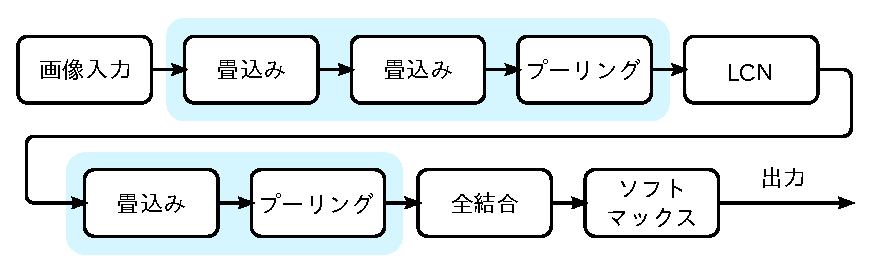
\includegraphics[clip,width=9cm]{fig/eps/structure.eps}
  \end{center}
  \caption{畳込みニューラルネットワークの構造}
\end{figure}

\begin{itemize}
\item 畳込み層(convolution layer)とプーリング層(pooling layer)が\\ペアでこの順に並び,このペアが複数回繰り返される
\item 畳込み層とプーリング層の後に,局所コントラスト正規化\\(local contrast normalization, LCN)層を挿入する場合がある
\item 畳込み層とプーリング層の繰り返しの後には,隣接層間ユニットが\\全結合した層が配置される
\item 目的がクラス分類であれば最終的な出力はソフトマックスを適用する
\end{itemize}
\end{frame}


%%%% 畳込みニューラルネットワークの構造 2 %%%%
\begin{frame}[fragile]\frametitle{畳込みニューラルネットワークの構造}

\begin{figure}[tb]
  \begin{center}
    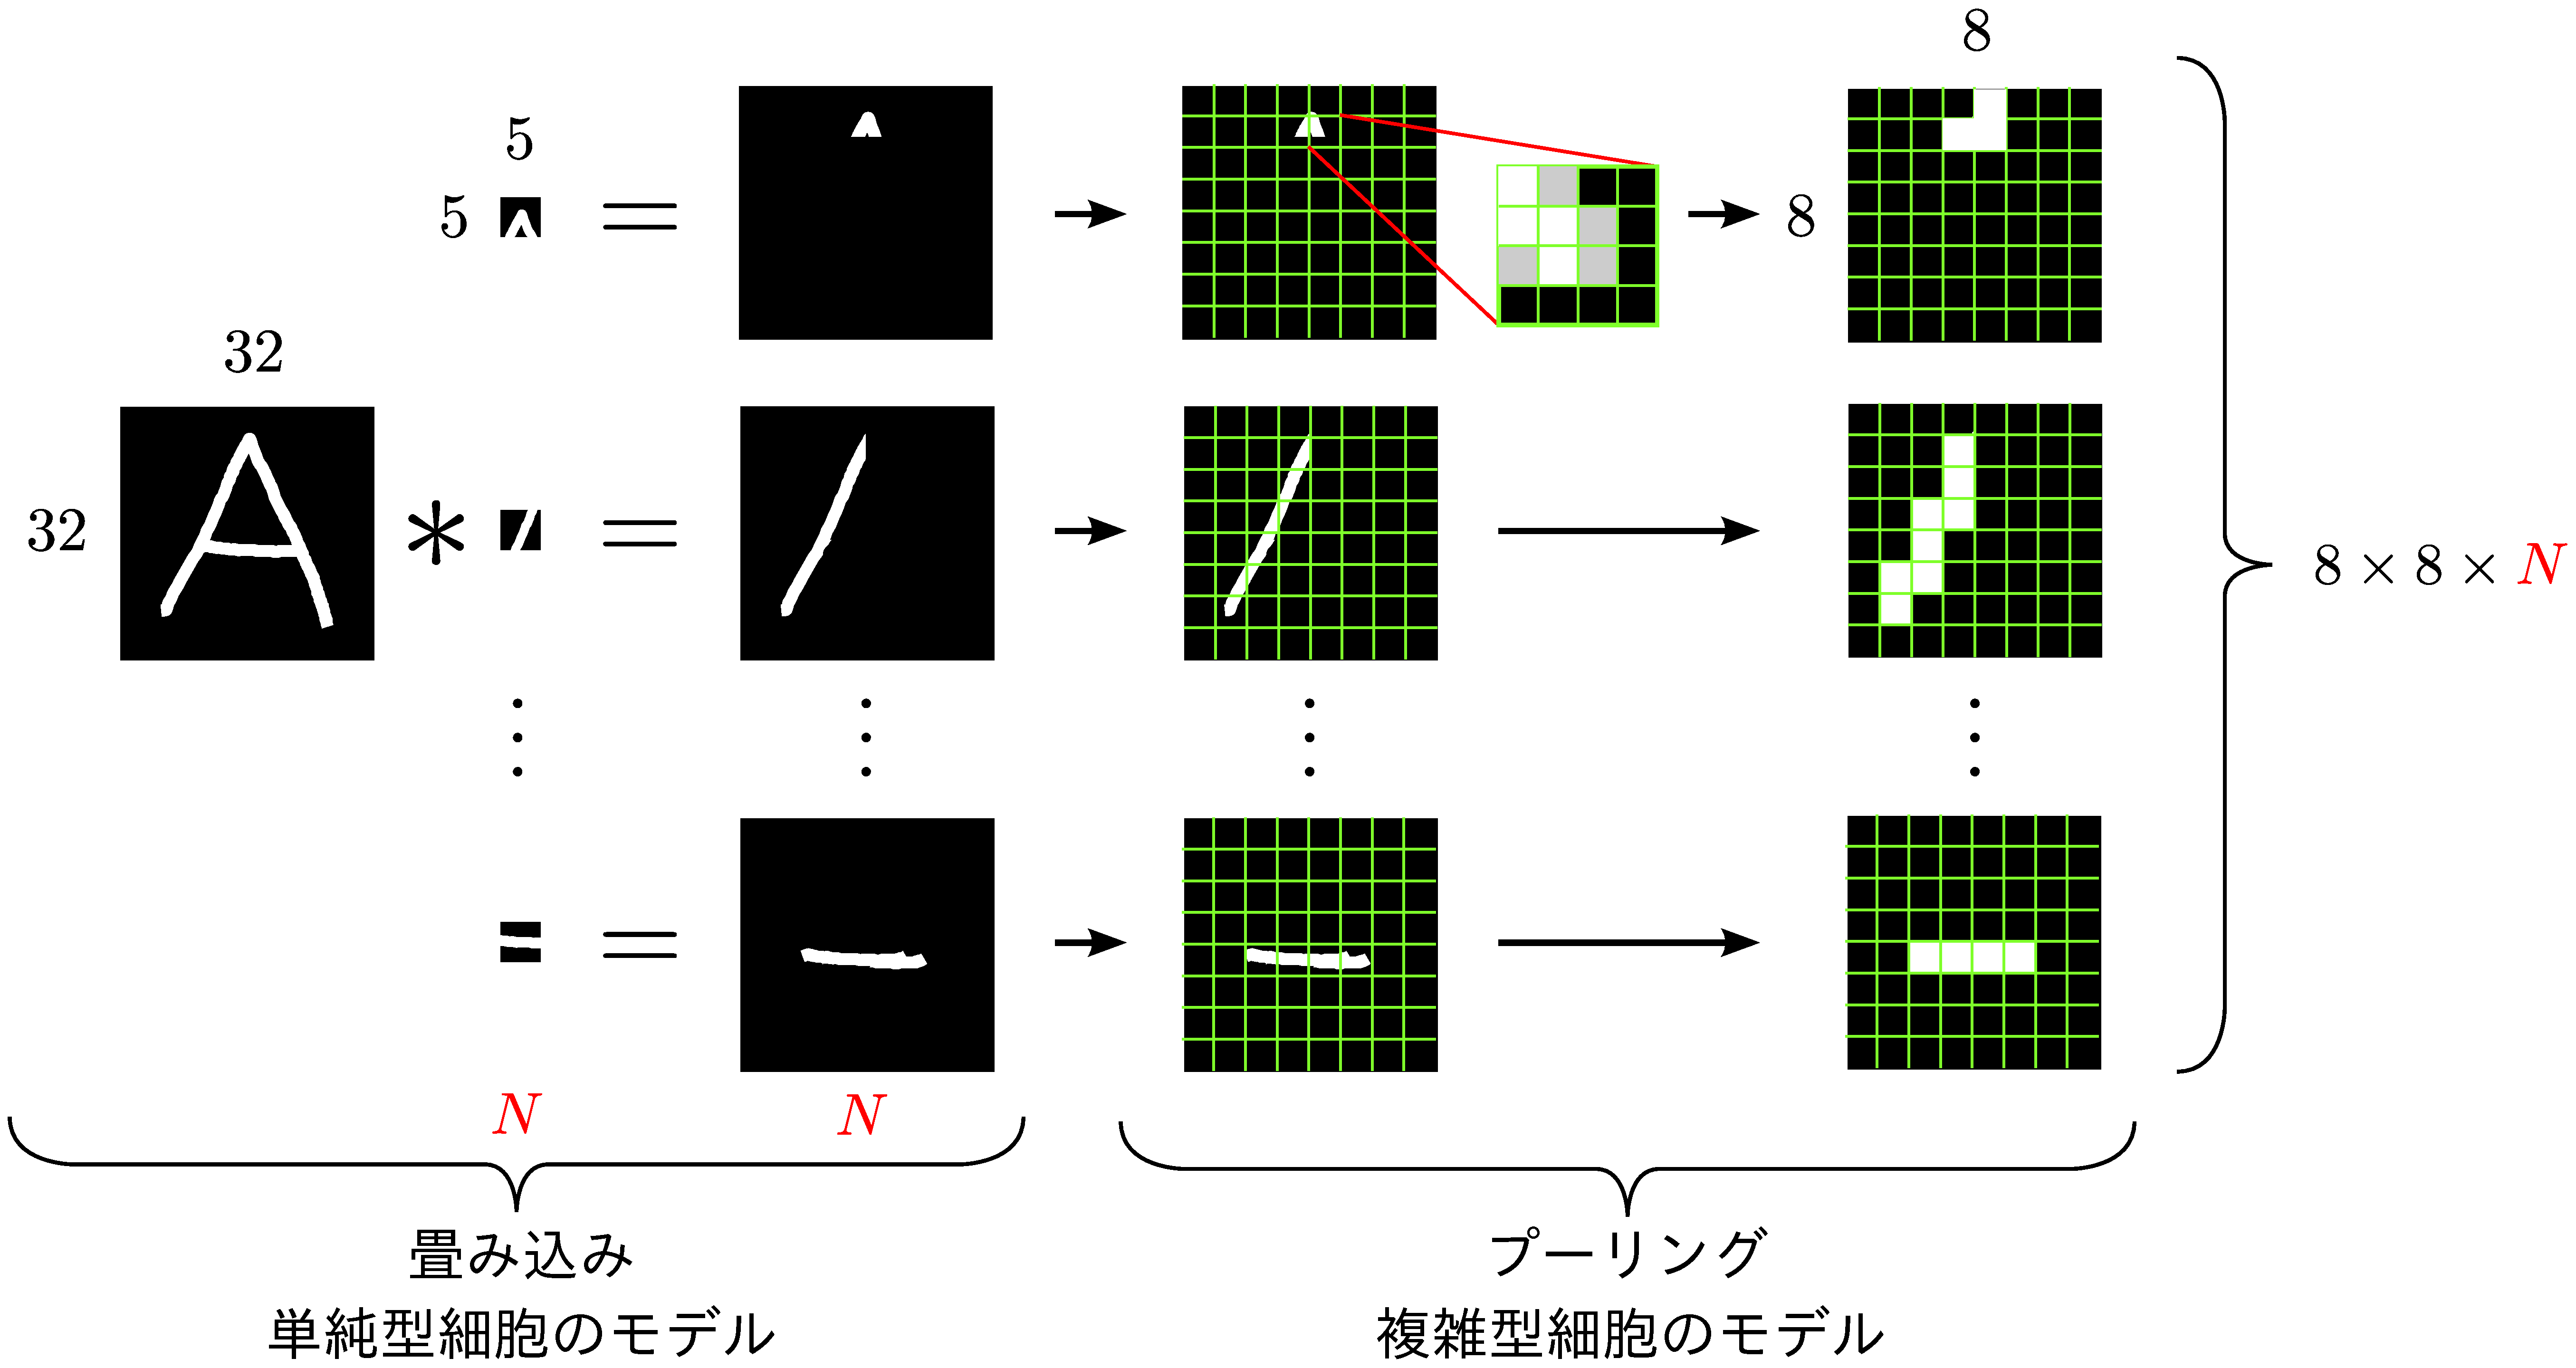
\includegraphics[clip,width=10cm]{fig/eps/conv_pool.eps}
  \end{center}
  % \caption{畳込みニューラルネットワークの構造}
\end{figure}

\begin{block}{二層の働き}
\begin{itemize}
\item 畳込み層はフィルタが表す特徴を入力から抽出する
\item プーリング層は抽出された特徴の位置感度を低下させる
\end{itemize}
\end{block}

\end{frame}



%%%% 畳み込み層%%%%
\begin{frame}[fragile]\frametitle{畳み込み層}

\begin{figure}[t]
 \centering
 \includegraphics[scale=0.25]{fig/eps/dl67.eps}
\end{figure}

\begin{itemize}
\item 各フィルタについて並列に計算され,$u_{ijm}$が出力される.
各チャンネルについて並列に画像とフィルタの畳み込みを行い全チャンネルにわたり加算する.

\begin{equation}
  u_{ijm} = \sum_{p=0}^{K-1} \sum_{q=0}^{H-1} \sum_{q=0}^{H-1} z_{i+p,j+q,k}^{(l-1)} h_{pqkm}+b_{ijm}
\end{equation}

\end{itemize}
\end{frame}

%%%% ogata %%%%
% \begin{frame}[fragile]\frametitle{畳み込み層}
% \begin{block}{活性化関数への適応}
% \begin{equation}
%  z_{ijm}=f(u_{ijm})
% \end{equation}
% \end{block}

% 式(1), (2)は,層間に特別な構造を持つ単層ネットワークとして表現できる.
% \begin{itemize}
%  \item 入力のユニット数:$W\times W\times K$
%  \item 出力のユニット数:$W\times W\times M$
% \end{itemize}

% 畳み込みの計算の局所性により,出力層のユニット1つは入力層の
% $W\times W\times K$個のユニットとのみ結合する.
% \begin{itemize}
%  \item その時の重みがフィルタ係数$h_{pqkm}$
%  \item 同一チャネルの全ユニットで共有されるため\\
% 			 重み共有(weigh sharing, weight tying)と呼ばれる
% \end{itemize}
% \end{frame}


%%%% プーリング 1 %%%%
\begin{frame}[fragile]\frametitle{プーリング}
\begin{block}{プーリング}
プーリング層は通常,畳み込み層の直後に設置され,プーリング層は畳み込み層で抽出された特徴の位置
感度を低下させる働きがある.
\end{block}
サイズ$W \times W \times K$の入力画像上で画素$(i,j)$を中心とする$H\times H$の正方領域$P_{ij}$をとり,$P_{ij}$内の画素についてチャネル$k$ごとに独立に,$H^2$個ある画素値を使って1つの画素値$u_{ijk}$を求める. 最大プーリングや平均プーリングなどがある.
\begin{figure}[bt]
 \centering
 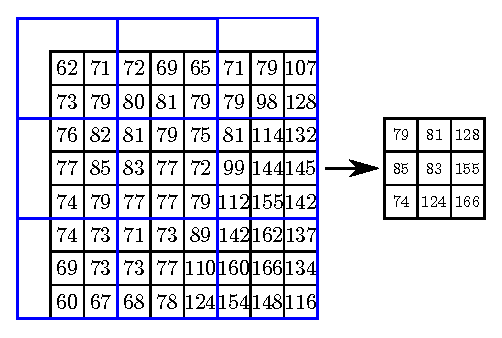
\includegraphics[scale = 0.6]{fig/eps/pooling.eps}
 \caption{プーリングの例.プーリングサイズ$3\times 3$,ストライド$s=3$,ゼロパディングで最大プーリングを行った場合}
\end{figure}
\end{frame}

% %%%% 局所コントラスト正規化%%%%
% \begin{frame}[fragile]\frametitle{局所コントラスト正規化}

%  \begin{block}{局所コントラスト正規化}
%  画像の中から対象物を捉えるための、画像の濃淡を正規化する方法の一種
%  \end{block}

%  \begin{itemize}
%   \item 1つの層だけでこの処理が可能
%   \item 畳み込みネットに組み込むことが可能
%   \item 層の重みは固定され,学習の対象となるパラメータはない
%   \item 減算正規化と除算正規化の2種類がある

%  \end{itemize}
% \end{frame}

%%%%勾配の計算%%%%
\begin{frame}[fragile]\frametitle{勾配の計算}

 \begin{block}{畳み込み層の計算式}
  \begin{equation}
   u^{(l)} = W^{(l)} u^{(l-1)} + b^{(l)}
  \end{equation}
  \begin{equation}
   z^{(l)} = f^{(l)} (u)
  \end{equation}
 \end{block}

 \begin{itemize}
  \item 逆伝播の計算も多層パーセプトロンのときと基本的に同じ
  \item 同じフィルタの係数が何度も現れてしまう
 \end{itemize}

 \begin{block}{重みの計算式}
  \begin{equation}
   W_{ji} = t_{ji}^{T} h
  \end{equation}
 \end{block}

 \begin{itemize}
  \item $h$:フィルタの係数$h_{pqkm}$を適当な順に並べたベクトル
  \item $t_{ji}$:$h$と同じ長さで,$h$との内積が重み$w_{ji}$を与えるベクトル
 \end{itemize}

\end{frame}

%%%% ogata %%%%
\begin{frame}[fragile]\frametitle{勾配の計算}
% 層$l$のデルタを$\delta^{(l)}$とし,全結合層に対する勾配計算の式を
% 形式的に適応したときの層の重み${\bf W}={\bf W}^{(l)}$の勾配

 \begin{block}{層$l$の重みの勾配}
  \begin{equation}
  \partial{\bf W}= {\bf \delta}^{(l)}{\bf z}^{{(l-1)}^\top}
  \end{equation}
 \end{block}

 \begin{itemize}
	\item ${\bf \delta}^{(l)}$: 層$l$のデルタ
	\item ${\bf z}^{(l-1)}$: $l-1$層からの出力
 \end{itemize}

${\bf W}$の多くの成分はもともと0であり.そうで
ない成分も重み共有により同じ変数(フィルタの係数)に対応する.そこでフィ
ルタの係数$\bf{h}$についての勾配$\partial{\bf h}$に変形する必要がある.

 \begin{block}{フィルタ係数についての勾配成分}
	\begin{equation}
 (\partial{\bf h})_r =\sum_{i,j}^{}({\bf T}_r\odot\partial{\bf W})_{ji}
	\end{equation}
 \end{block}

\begin{itemize}
 \item $\odot$ : 成分ごとの積
 \item $\sum_{}^{}$: 行列の全成分の和
\end{itemize}

\end{frame}

% \begin{frame}[fragile]\frametitle{勾配の計算}
% プーリング層には学習の対象となるパラメータはないので,勾配計算は必要ない
% が,さらに下層に伝えるデルタの逆伝播計算は必要である.

% \begin{block}{平均プーリング層の逆伝播計算}
%  \begin{equation}
%  w_{ji}^{(l+1)} =
% 	\begin{cases}
%     \frac{1}{H^2} & (\text {if}  \  i\in{P_j}) \\
%     0 & (\text{otherwise})
%   \end{cases}
%  \end{equation}
% \end{block}

% \begin{itemize}
%  \item $P_{j}$ : 層$l+1$のユニット$j$のサイズ$H \times H$の受容野
%  \item 順伝播時のプーリングの結果により重みが変化する
%  \item 逆伝播計算では最大値を返したユニットにデルタがそのまま伝えられる
% \end{itemize}

% \end{frame}

% %%%%Dropout%%%%
% \begin{frame}\frametitle{ドロップアウト}
%  \begin{block}{ドロップアウト}
%   多層ネットワークのユニットを確率的に選別して学習する方法
%  \end{block}
%  \begin{itemize}
%   \item 自由度を下げて,過適合を避ける
%   \item 複数のネットワークの平均をとり,精度が向上する
%  \end{itemize}
% \begin{figure}[tb]
%   \begin{center}
%     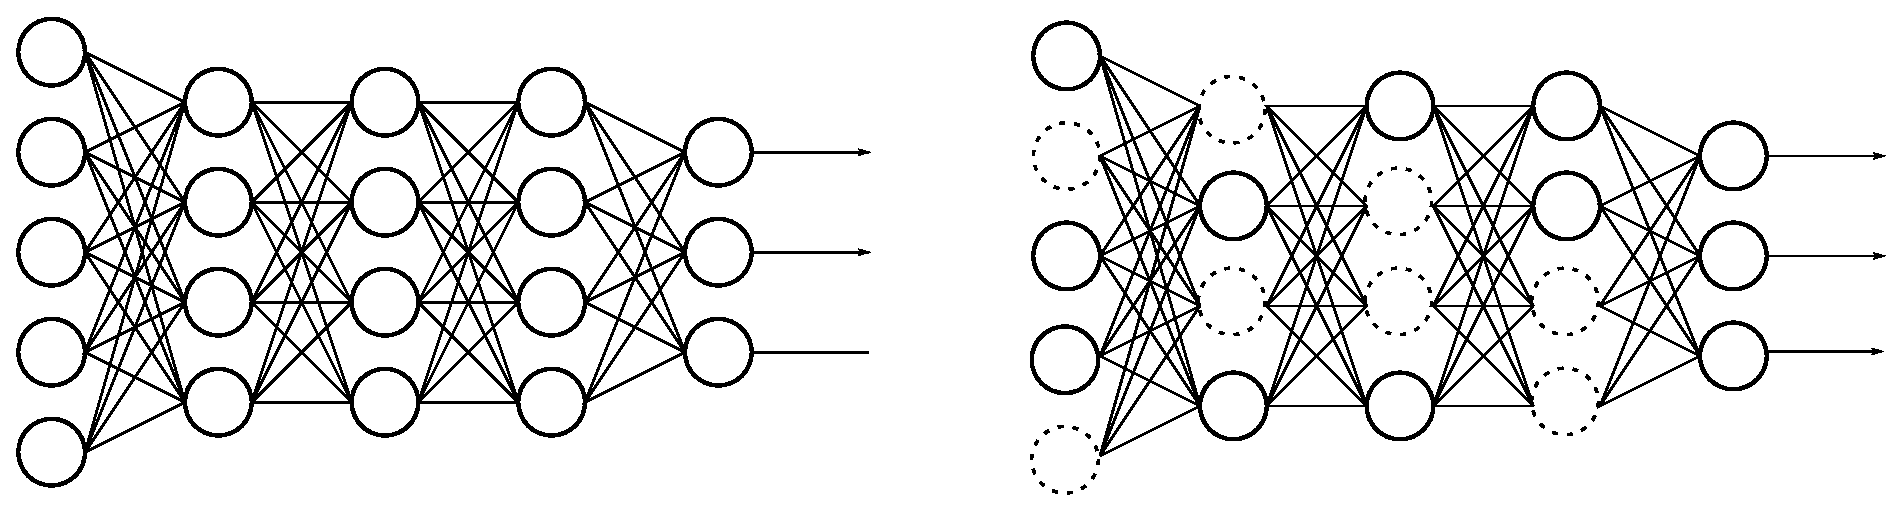
\includegraphics[clip,width=7cm]{./fig/eps/dropout1.eps}
%   \end{center}
%   \caption{ドロップアウト($p$=0.5程度)}
%   \label{fig: ドロップアウト(p=0.5程度)}
% \end{figure}
% \vspace{-0.5cm}
%  〜学習時〜
%  \begin{itemize}
%   \item 中間層の各層と入力層のユニットをある割合$p$でランダムに選出し,それ以外は無効化 $\rightarrow$ いつも通り最適化
%  \end{itemize}
%  〜学習終了後〜
%  \begin{itemize}
%   \item 無効化された層の出力を$p$倍し,すべてのユニットで逆伝播計算
%  \end{itemize}
% \end{frame}

% %%%% 少女時代のメンバー識別でドロップアウトを試す %%%%
% \begin{frame}\frametitle{Caffeでドロップアウトを試す}
% \begin{itemize}
%   \item 今まではアニメーション(ラブライブ!)を切り出して学習を行って,性能評価を行った.
%   \item ラブライブ!のキャラクター識別は短い学習時間で高い学習精度を得ることができた.
%   \item 学習の結果を解析したが,過学習の傾向は見られなかった.
%   \item そこで次の課題として実在する人物の識別を行うことを目指し,韓国の女性アイドルグループ(少女時代)のメンバーの識別を試みた.
% \end{itemize}
% \begin{figure}[htbp]
%   \begin{center}
%     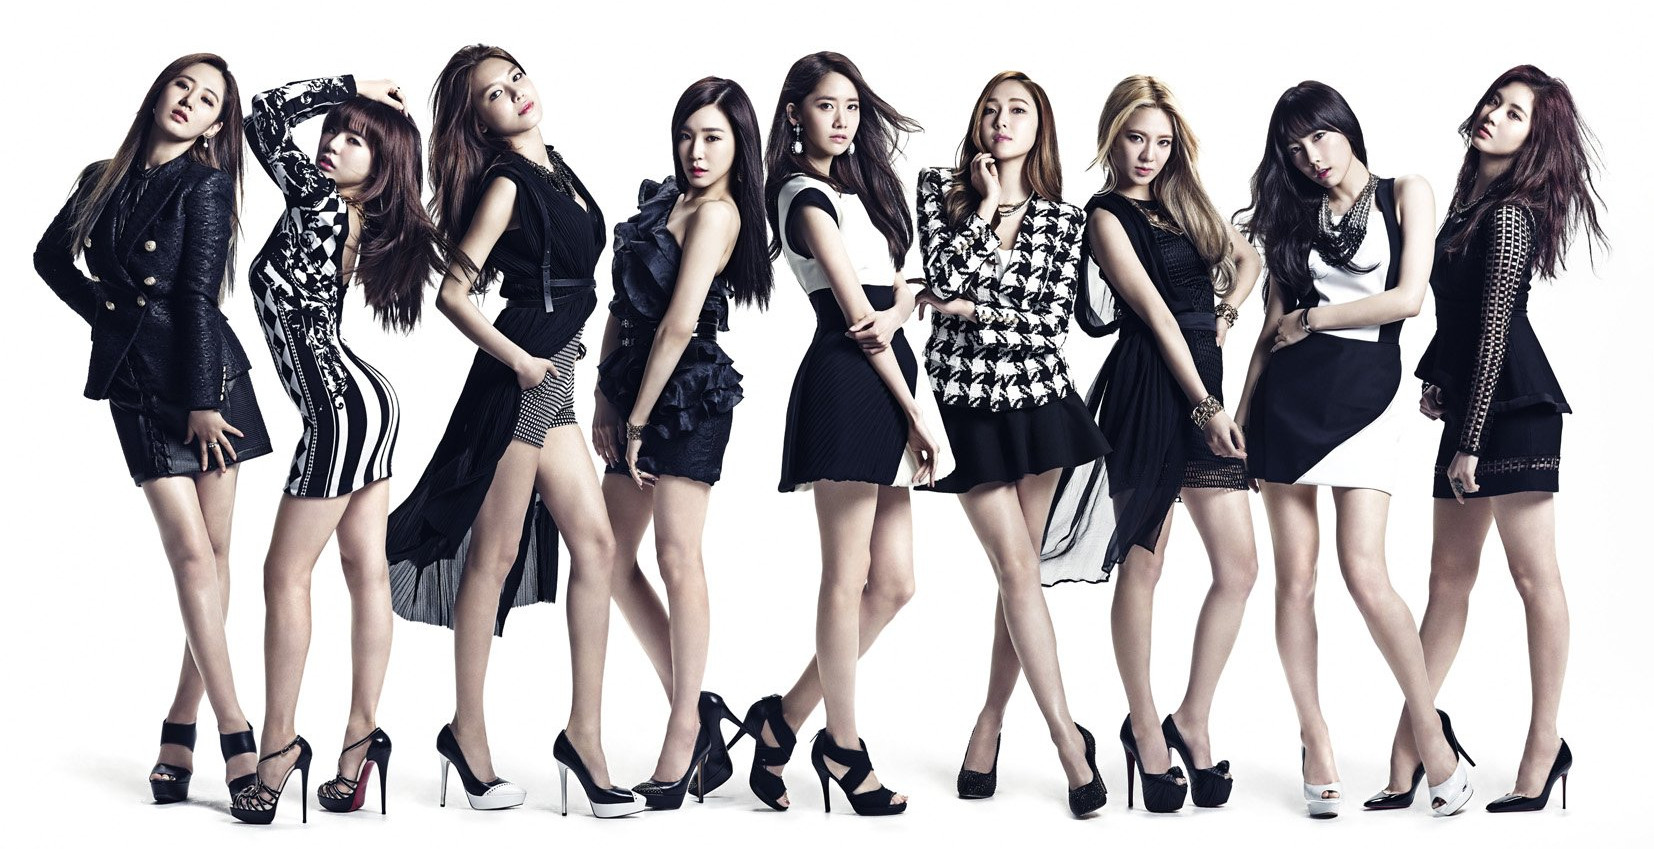
\includegraphics[clip,width=9cm,bb=0 0 1654 849]{./fig/jpg/snsd.jpg}
%   \end{center}
% \end{figure}

% \end{frame}

% %%%% 少女時代のメンバー識別でドロップアウトを試す %%%%
% \begin{frame}[fragile]\frametitle{Caffeでドロップアウトを試す}
% ラブライブ!の学習でも用いた通常のCifar10のモデルで学習を行った結果
% \begin{figure}[tb]
%   \begin{center}
%     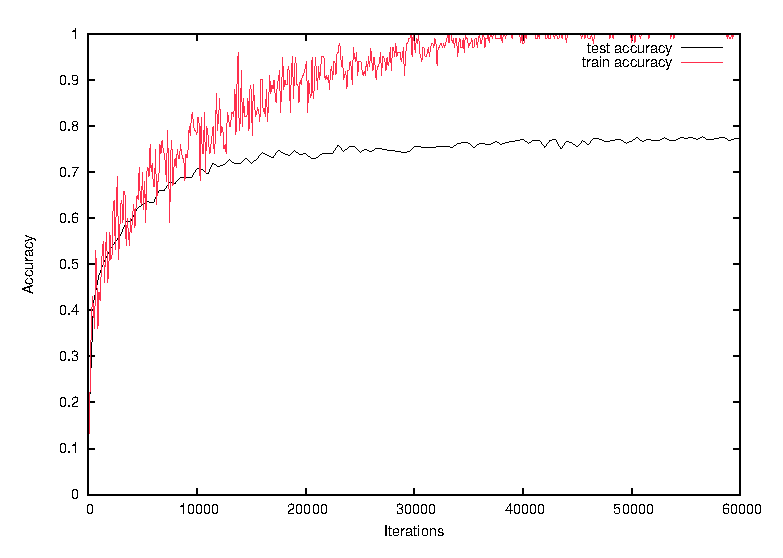
\includegraphics[clip,width=8cm]{./fig/eps/overtraining.eps}
%   \end{center}
%   \caption{通常のCifar10のモデルで実行した学習結果}
% \end{figure}
% \end{frame}

% %%%% 少女時代のメンバー識別でドロップアウトを試す %%%%
% \begin{frame}[fragile]\frametitle{Caffeでドロップアウトを試す}
% \begin{alertblock}{結果}
% 訓練データに関しての精度は$1$に収束しているが,テストデータに関しては精度は$77\%$程度である.
% \end{alertblock}
% \begin{itemize}
%   \item 理論に関する発表で説明したドロップアウトを導入し,過学習の回避を試みる.
%   \item ドロップアウトのユニットを追加するだけでなく,\\過学習が起きる原因となる学習データの不足が考えられるため単純にデータセットを増やす以外の方法を模索.
%   \item 入力として使うデータセットをランダムにクロップし入力データとして学習を行う方法と,入力データをランダムで左右反転させる方法
% \end{itemize}
% \end{frame}

% %%%% 少女時代のメンバー識別でドロップアウトを試す %%%%
% \begin{frame}[fragile]\frametitle{Caffeでドロップアウトを試す}
% \begin{figure}[tb]
%   \begin{center}
%     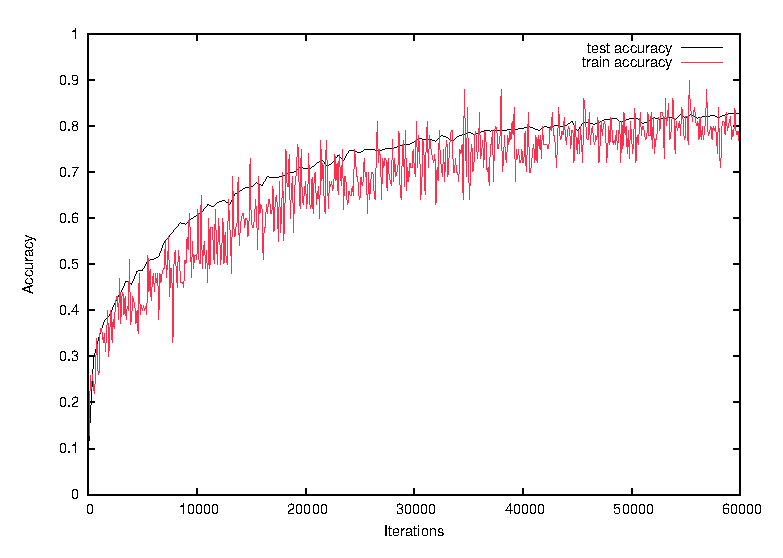
\includegraphics[clip,width=8cm]{./fig/eps/dropout.eps}
%   \end{center}
% \end{figure}
% \begin{block}{工夫の結果}
% 過学習を抑えることに成功.
% 最終的なテストデータに関する精度は$88\%$と通常のCifar10のモデルを使用した場合よりも精度向上が見られた.
% \end{block}
% \end{frame}

\begin{frame}\frametitle{caffeによる学習と認識}
\begin{itemize}
\item アニメキャラクターの認識(ラブライブ!$\cdots$ 9人のキャラクター$+$etc)
\item アイドルグループの顔認識(少女時代のメンバー$\cdots$ 9人$+$etc)
\item 手書きひらがな文字認識(ひらがな48文字$+$濁音20文字$+$半濁音5文字$=$73文字)
\end{itemize}
\begin{figure}[t]
 \begin{minipage}{0.3\hsize}
  \centering
  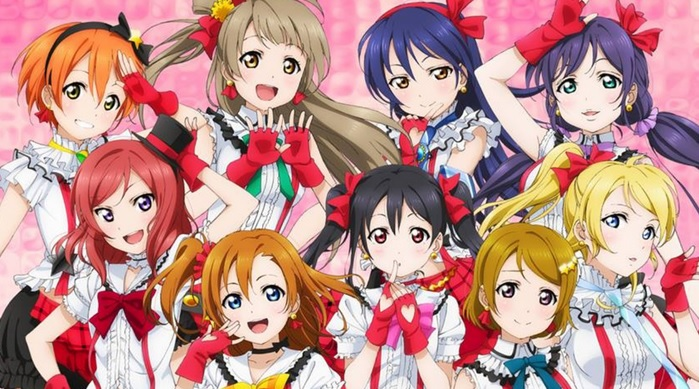
\includegraphics[width=30mm]{./fig/jpg/lovelive.jpg} \\
  \text{ラブライブ!}
 \end{minipage}
 \begin{minipage}{0.3\hsize}
  \centering
  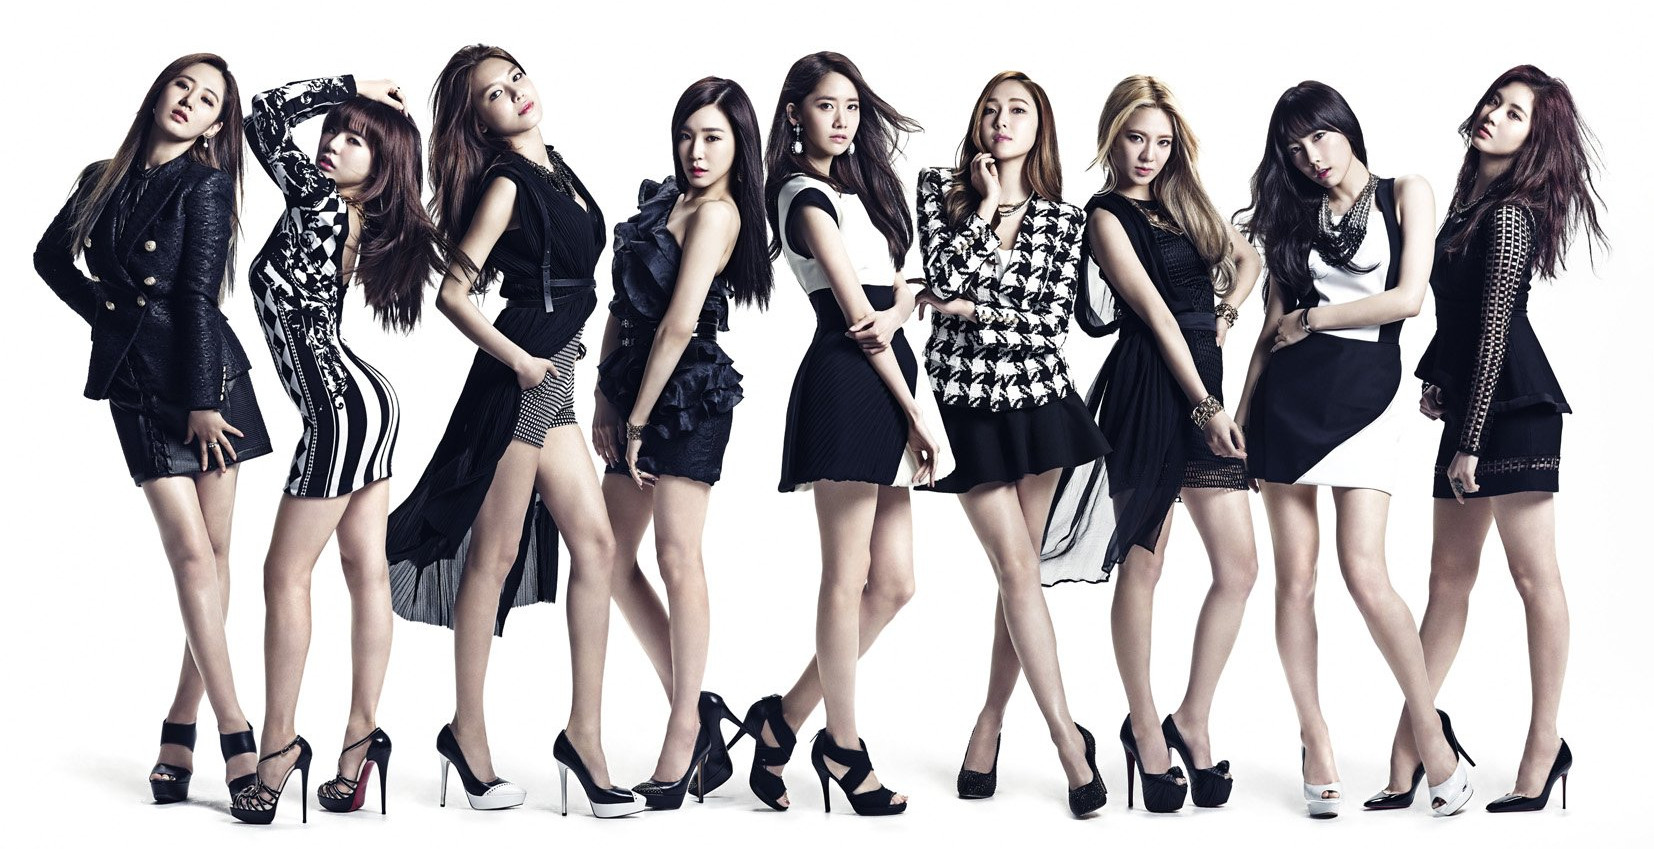
\includegraphics[width=40mm]{./fig/jpg/snsd.jpg}\\
  \text{少女時代}
 \end{minipage}
 \begin{minipage}{0.3\hsize}
  \centering
  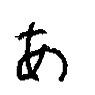
\includegraphics[width=20mm]{./fig/jpg/a.jpg}\\
  \text{手書き文字}
 \end{minipage}
\end{figure}
\end{frame}

\begin{frame}\frametitle{データセットと学習器}
\begin{itemize}
\item アニメキャラクターの認識\\
    各キャラクターに2500枚$\sim$4000枚と負例約9000枚
\item アイドルグループの顔認識(少女時代のメンバー$\cdots$ 9人$+$etc)\\
    各メンバーに1000枚$\sim$2500枚と負例約3500枚
\item 手書きひらがな文字認識(ひらがな48文字$+$濁音20文字$+$半濁音5文字$=$73文字)\\
    各文字に180枚
\end{itemize}
学習器にはcifar10のフルソルバーを使用した.
\begin{figure}[ht]
 \centering
 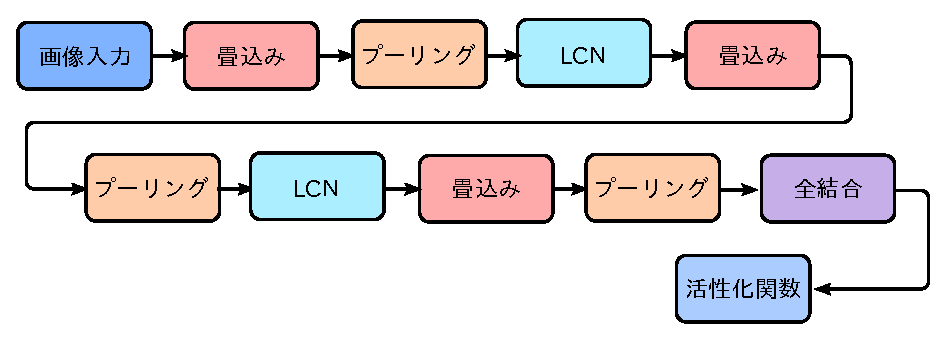
\includegraphics[scale=0.7]{fig/eps/cifar10Net_structure.eps}
\end{figure}
\end{frame}

\begin{frame}\frametitle{学習結果(ラブライブ!)}
 \begin{figure}[ht]
 \centering
 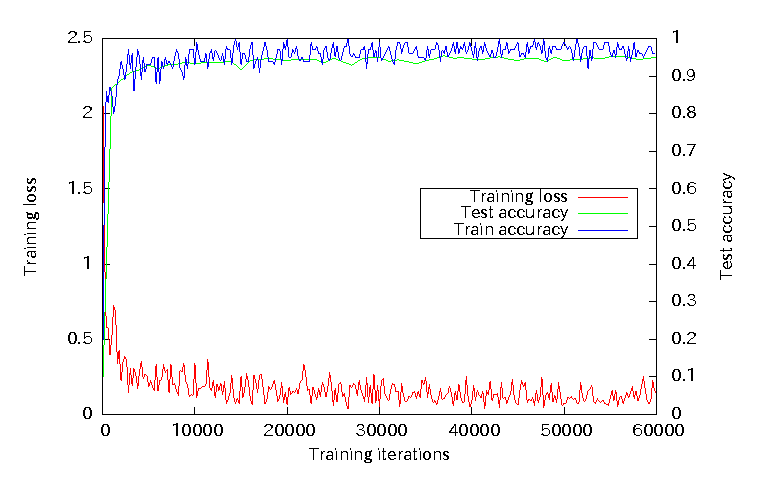
\includegraphics[scale=0.85]{fig/eps/result_train_test_lovelive_full.eps}
 \caption{損失関数の値と精度}
\end{figure}
\end{frame}

\begin{frame}\frametitle{識別結果}
\begin{figure}[t]
  \begin{center}
    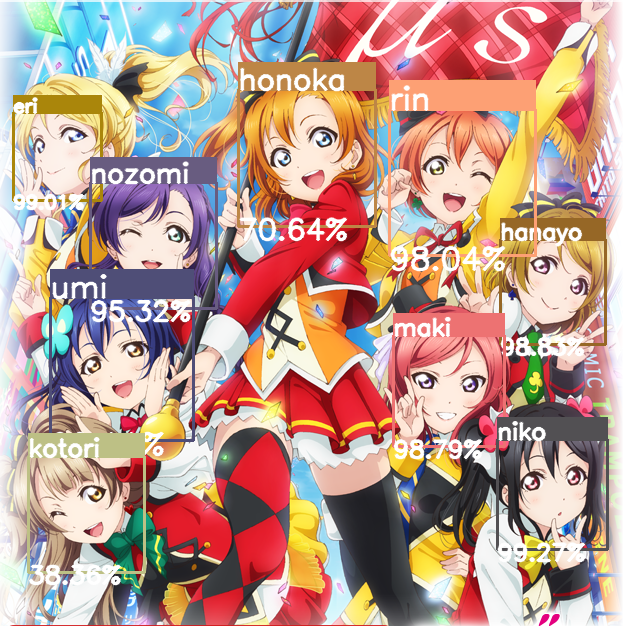
\includegraphics[clip,width=7cm, bb = 0 0 624 626]{./fig/png/lovelive_classify.png}\\
  \end{center}
  \text{識別器を用いた識別結果}
\end{figure}
\end{frame}

\begin{frame}\frametitle{アニメキャラクター認識時の中間層出力}
\begin{figure}[t]
  \centering
  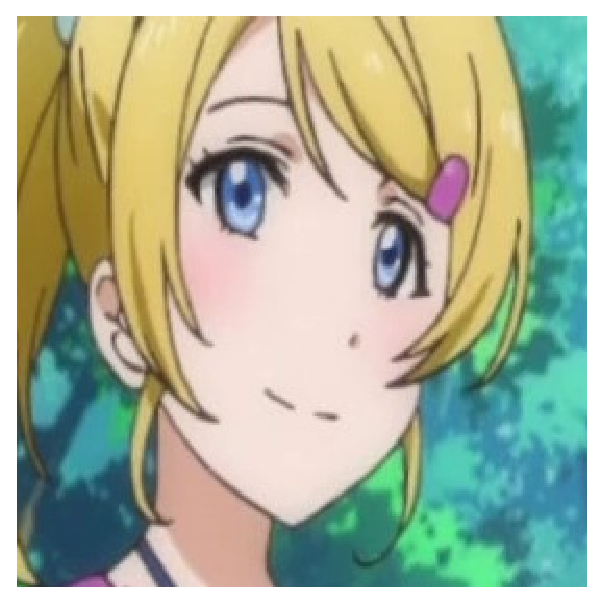
\includegraphics[clip,width=1.5cm]{./fig/eps/eri.eps}
\end{figure}
\begin{figure}[t]
 \begin{minipage}{0.45\hsize}
  \centering
  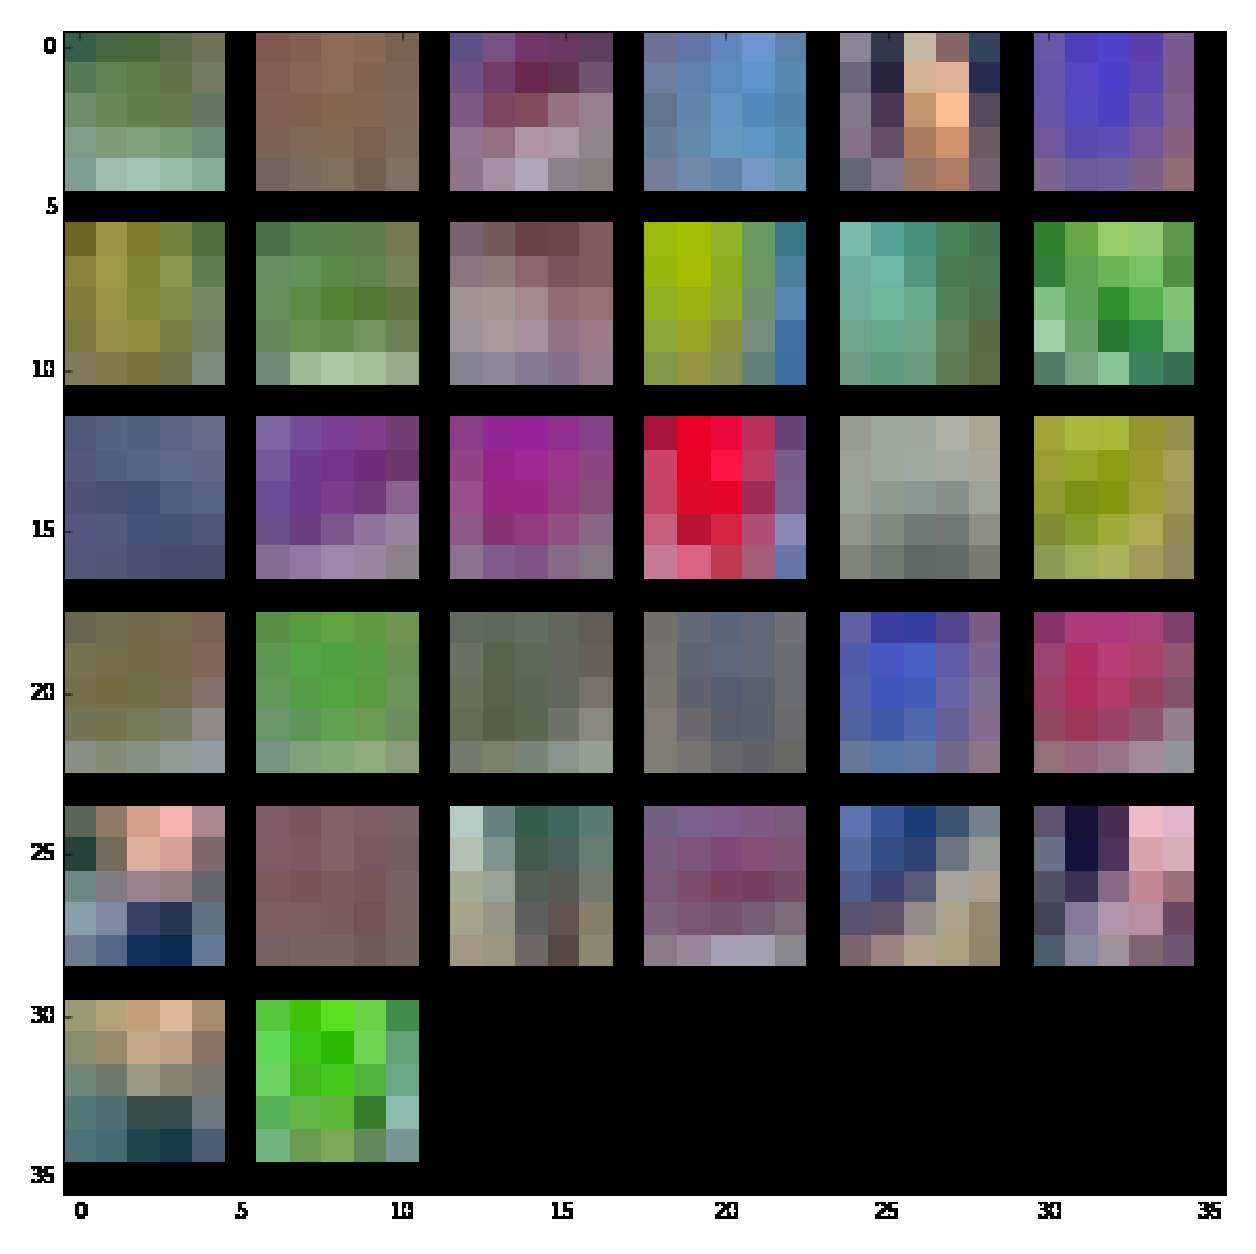
\includegraphics[width=50mm]{./fig/eps/filtereri.eps} \\
  \text{フィルタ}
 \end{minipage}
 \begin{minipage}{0.45\hsize}
  \centering
  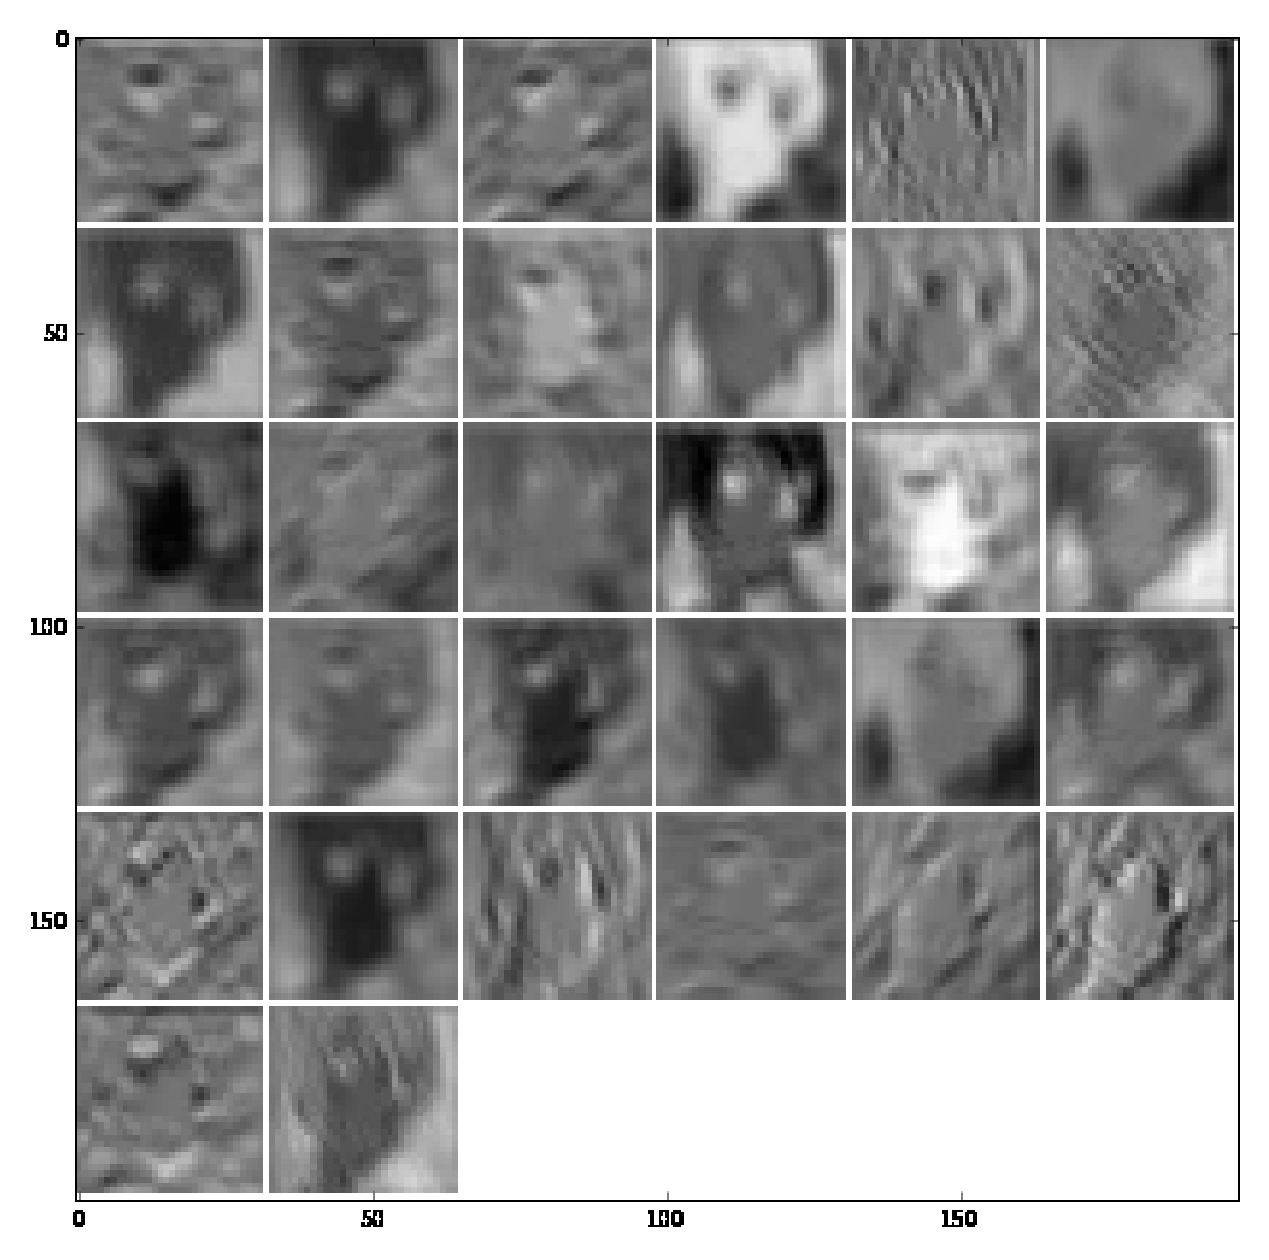
\includegraphics[width=50mm]{./fig/eps/outputeri.eps}\\
  \text{第一層目の出力}
 \end{minipage}
\end{figure}
\end{frame}

\begin{frame}\frametitle{学習結果(少女時代)}
ドロップアウトのユニットをCaffeの学習に取り込んだ結果
\begin{figure}[ht]
  \centering
  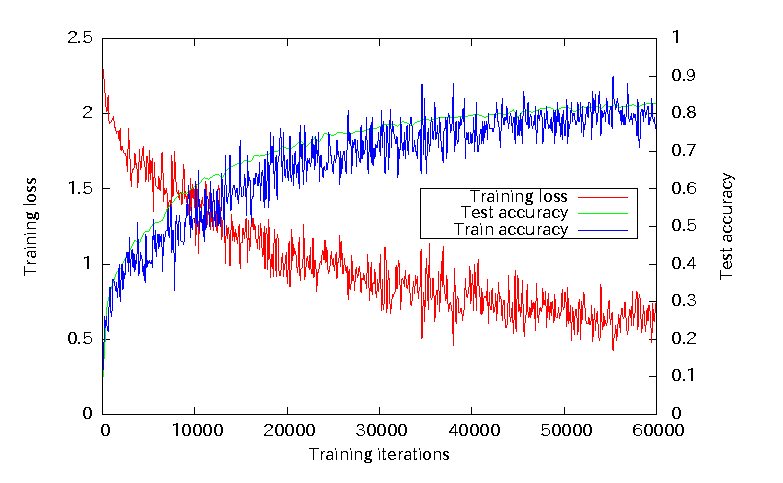
\includegraphics[scale=0.85]{fig/eps/result_dropout_test_graph_snsd.eps}
  \caption{損失関数の値と精度}
\end{figure}
\end{frame}

\begin{frame}\frametitle{識別結果}
\begin{figure}[t]
  \begin{center}
    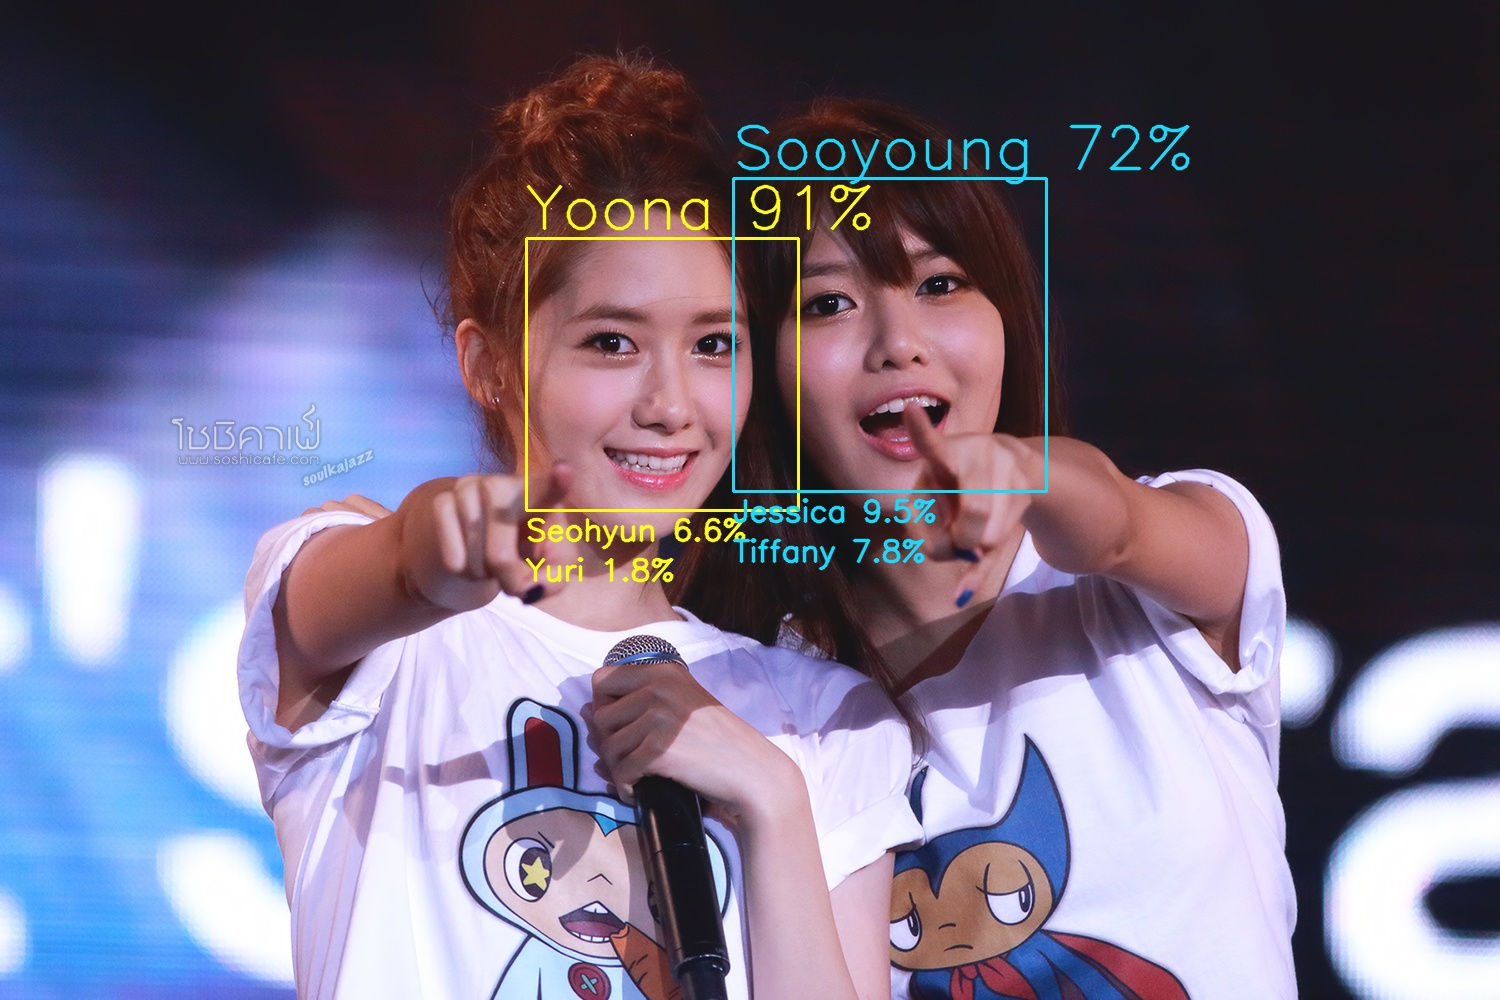
\includegraphics[clip,width=10cm, bb = 0 0 1500 1000]{./fig/jpg/yoona_sooyoung.jpg}\\
  \end{center}
  \text{識別器を用いた識別結果}
\end{figure}
\end{frame}

\begin{frame}\frametitle{認識時の中間層出力}
\begin{figure}[t]
  \centering
  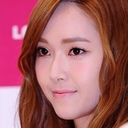
\includegraphics[clip,width=1.5cm, bb = 0 0 128 128]{./fig/png/jessica_0010.jpg}
\end{figure}
\begin{figure}[t]
 \begin{minipage}{0.45\hsize}
  \centering
  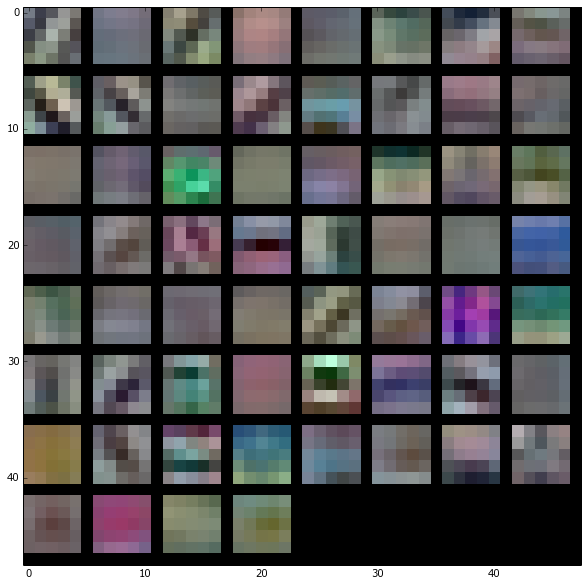
\includegraphics[width=50mm, bb = 0 0 588 586]{./fig/png/snsd_filter.png} \\
  \text{フィルタ}
 \end{minipage}
 \begin{minipage}{0.45\hsize}
  \centering
  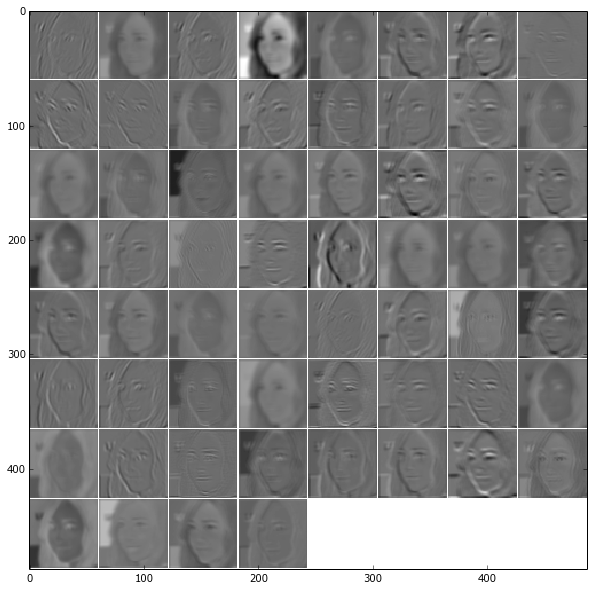
\includegraphics[width=50mm, bb = 0 0 594 590]{./fig/png/snsd_output.png}\\
  \text{第一層目の出力}
 \end{minipage}
\end{figure}
\end{frame}


\begin{frame}\frametitle{学習結果(手書き文字認識)}
 \begin{figure}[ht]
 \centering
 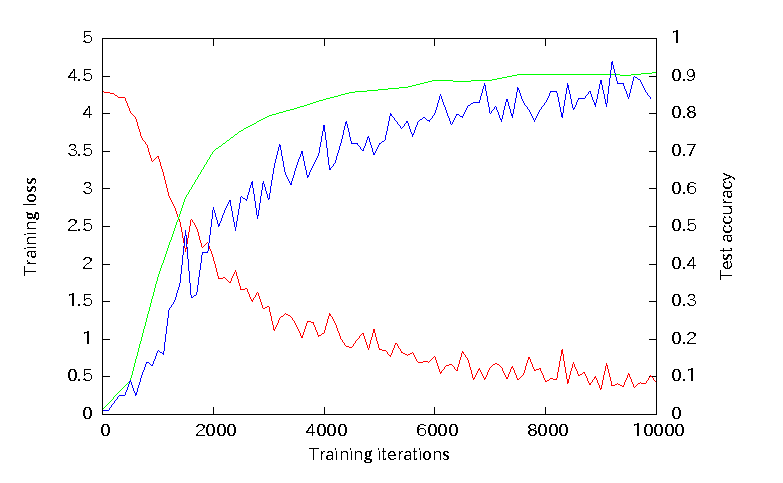
\includegraphics[scale=0.85]{fig/eps/result_train_test_tegaki_graph.eps}
 \caption{損失関数の値と精度}
\end{figure}
\end{frame}

\begin{frame}\frametitle{識別結果}
手書き文字認識用の簡単なアプリケーションの作成
\begin{figure}[t]
  \begin{center}
    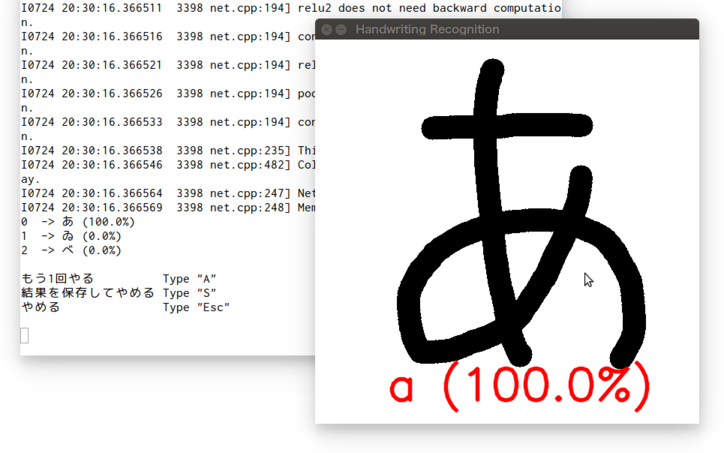
\includegraphics[clip,width=10cm, bb = 0 0 724 453]{./fig/png/tegaki_result.png}\\
  \end{center}
  \caption{Caffeを使った手書き文字認識}
\end{figure}
\end{frame}

\begin{frame}\frametitle{DEMO}
\centering
\includemovie[label=tegaki, controls, repeat, poster, startat=frame:1]{10mm}{10mm}{movie/handwriting_recognition.mp4}\large{手書き文字認識アプリケーション}\\

\includemovie[label=lovelive, controls, repeat, poster, startat=frame:1]{10mm}{10mm}{./movie/loveliveop.mp4}\large{動画に対する顔認識}
\end{frame}

% \begin{figure}[t]
%  \begin{minipage}{0.3\hsize}
%   \centering
%   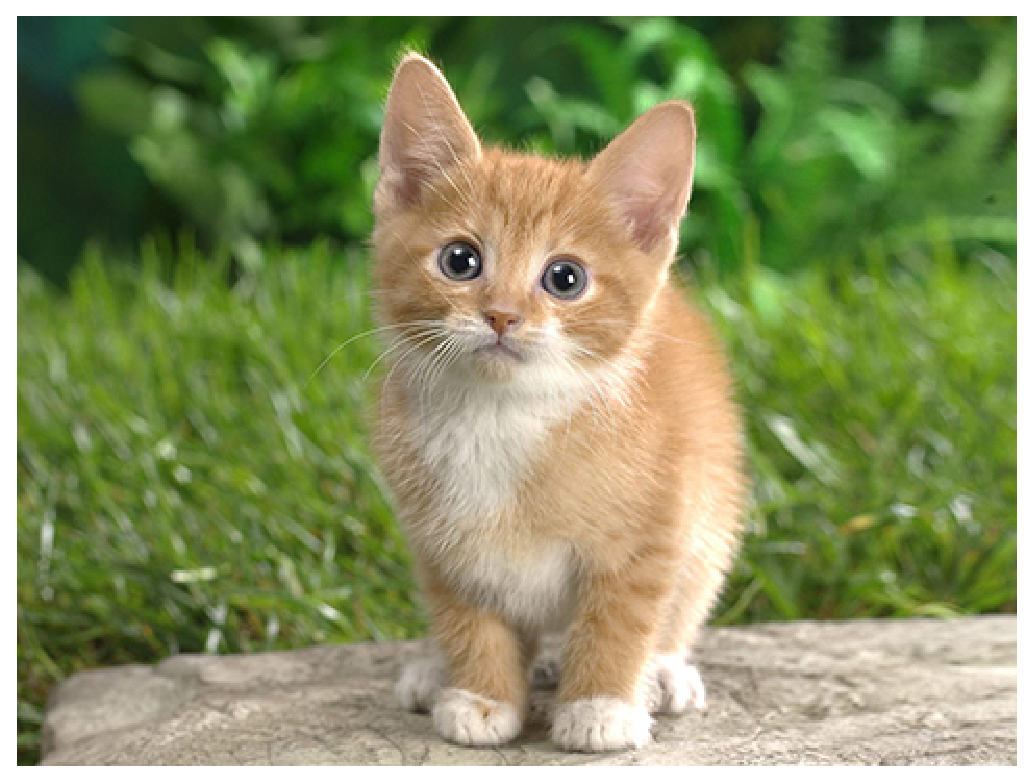
\includegraphics[width=30mm]{./figure/cat.eps}
%   \caption{cat.jpg}
%   \label{sample1}
%  \end{minipage}
%  \begin{minipage}{0.3\hsize}
%   \centering
%   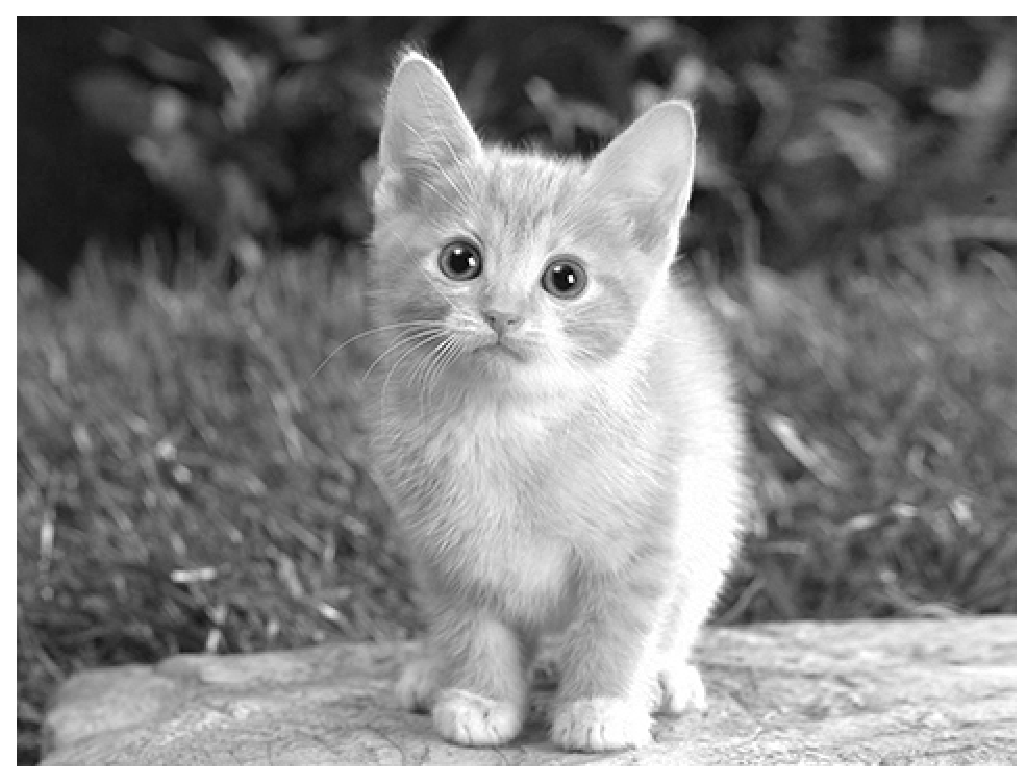
\includegraphics[width=30mm]{./figure/cat_gray.eps}
%   \caption{cat\_gray.jpg}
%   \label{sample2}
%  \end{minipage}
%  \begin{minipage}{0.3\hsize}
%   \centering
%   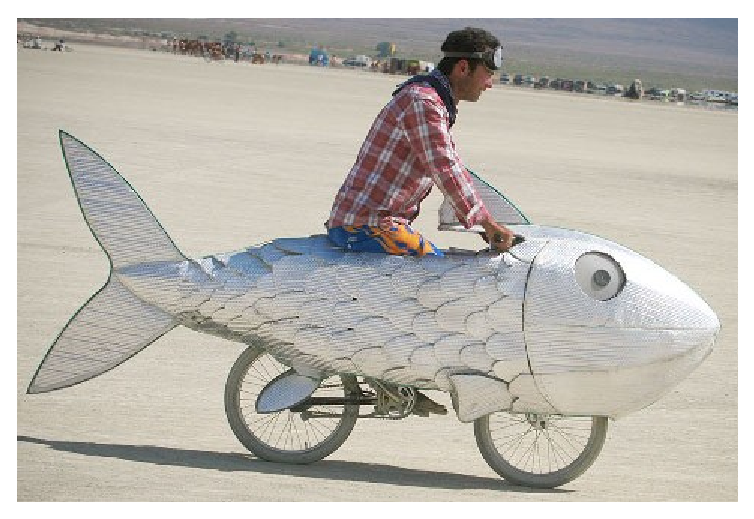
\includegraphics[width=30mm]{./figure/fish-bike.eps}
%   \caption{fish-bike.jpg}
%   \label{sample3}
%  \end{minipage}
% \end{figure}
% \begin{exampleblock}{実行環境}
% \begin{itemize}
%  \item Ubuntu 14.04 LTS
%  \item Intel core i5-4440 3.10GHz$\times$4
%  \item RAM 16GB
% \end{itemize}
% \end{exampleblock}
% \end{frame}


% \section{具体例}

% \begin{frame}\frametitle{定理環境の例}
% \begin{theorem}[Fermat]
% $a^{p-1} \equiv 1 \pmod{p}$
% \end{theorem}
% \pause
% \begin{theorem}[Wilson]
% \begin{equation}
% (p-1)! \equiv 1 \pmod{p}
% \end{equation}
% \end{theorem}
% \end{frame}

% \begin{frame}<1-2>\frametitle{オーバーレイ}
% \onslide*<1>{
% \Large{これは1枚目です}
% }
% \onslide*<2>{
% これは2枚目です
% \begin{theorem}[Euclid]
% There is no largest prime number.
% \end{theorem}
% }
% \end{frame}

% \begin{frame}\frametitle{色もつけれるよ}
%   {\color{red} red}(\alert{alert}),
%   {\color{blue} blue}(\structure{structure}),
%   {\color{green} green},
%   {\color{cyan} cyan},
%   {\color{magenta} magenta},
%   {\color{yellow} yellow},
%   {\color{black} black},
%   {\color{darkgray} darkgray},
%   {\color{gray} gray},
%   {\color{lightgray} lightgray},
%   {\color{orange} orange},
%   {\color{violet} violet},
%   {\color{purple} purple},
%   {\color{brown} brown},
% \end{frame}

% \begin{frame}\frametitle{いろんなブロック}
% \begin{block}{ブロック}
% これは普通のブロックです
% \end{block}

% \begin{alertblock}{警告ブロック}
% 警告!これは警告ブロックだ!
% \end{alertblock}

% \begin{exampleblock}{例ブロック}
% 例えば、こんなブロックです。
% \end{exampleblock}
% \end{frame}

% \begin{frame}<1-2>\frametitle{画像も貼れるよ}
% \onslide*<1>{
% このように画像を貼れるよ
% %\begin{figure}[htb]
% %\centering
% %\includegraphics[width=12cm,clip]{dummygraph.pdf}
% %\caption{$f(x)=e^{-\frac{x}{10}}\sin(x)$}
% %\end{figure}%
% }
% \onslide*<2>{
% 画像や表は各自用意してね
% %\begin{figure}[htb]
% %\centering
% %\includegraphics[width=8cm,clip]{sym4.pdf}
% %\caption{Cayley graph of $\mathfrak{S}_{4}$}
% %\end{figure}%
% }
% \end{frame}

% \begin{frame}\frametitle{まとめ}
% \LARGE{大事なのは中身です!}
% \end{frame}

% \begin{frame}\frametitle{}
% {\Large ありがとうございました}
% \end{frame}
% \appendix

\newcounter{finalframe}
\setcounter{finalframe}{\value{framenumber}}

% \begin{frame}[containsverbatim]\frametitle{dvipngの使い方(1)}
% \begin{block}{この様なファイルを用意する}
% \tiny{
% \begin{verbatim*}
% \documentclass[43pt]{jsarticle}
% \usepackage{amsmath}
% \usepackage{lmodern}
% \pagestyle{empty}
% \begin{document}
% \begin{equation*}
% \sum_{k=0}^{\infty} \frac{(2k)!}{2^{2k}(k!)^2} \frac{1}{2k+1}=\frac{\pi}{2}
% \end{equation*}
% \end{document}
% \end{verbatim*}
% }
% \end{block}
% \end{frame}

% \begin{frame}[containsverbatim]\frametitle{dvipngの使い方(2)}
% \begin{block}{使い方(コマンドライン)}
% \scriptsize{
% \begin{verbatim*}
% latex dvipng-sample.tex
% dvipng dvipng-sample.dvi -T tight -bd 1000
% \end{verbatim*}
% }
% \end{block}
% \end{frame}
\setcounter{framenumber}{\value{finalframe}}
\end{document}